\section{Conclusion}
\begin{itemize}
  \item Kelvin-Helmholtz and Holmboe modes were investigated
  \item More complicated problem requires computational technique
  \item 3D Evolution by Smyth and Winters \cite{Smyth}
\end{itemize}
\begin{figure}[htpb]
  \centering
  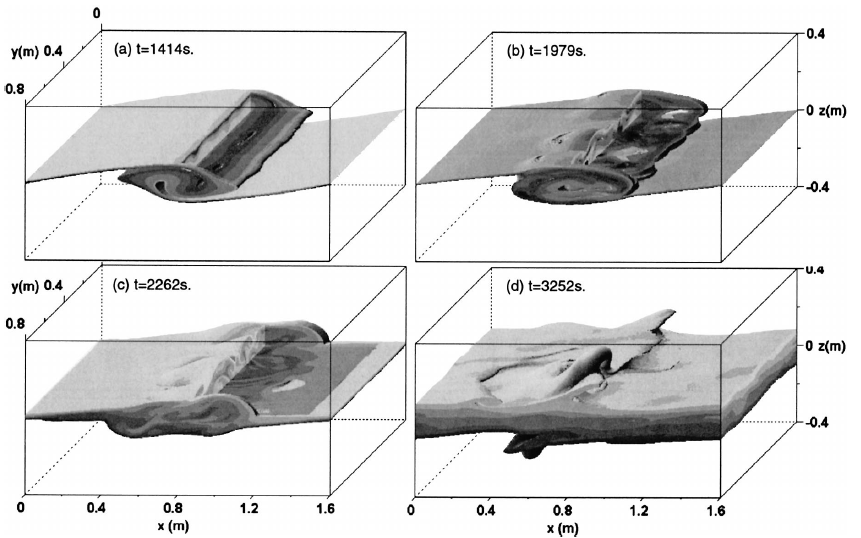
\includegraphics[width=0.9\textheight]{kh3.png}\\
  \caption{Time evolution for a Kelvin-Helmholtz mode (Smyth and Winters \cite{Smyth})}\label{kh3}
\end{figure}
\begin{figure}[htpb]
  \centering
  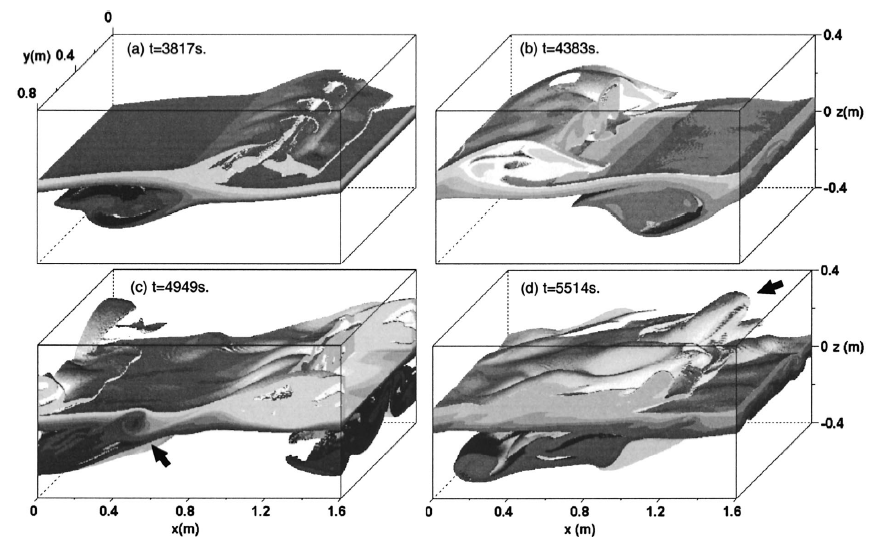
\includegraphics[width=0.9\textheight]{ho5.png}\\
  \caption{Time evolution for a Holmboe mode (Smyth and Winters \cite{Smyth})}\label{ho5}
\end{figure}
